SAND is an application layer network protocol on top of the TCP/IP stack. It 
makes use of a worldwide P2P network to allow anonymously distributing files on 
the internet.

It can additionally use UPnP to programmatically add a port mapping to the 
Internet Gateway Device. This will allow incoming messages on the port on which 
the client application is listening if the device is sitting behind a NAT 
capable gateway. Other mechanisms for NAT traversal can be used as well, 
depending on the protocol implementation.

The protocol consists of a number of messages (also called requests), which may 
or may not receive a reply, depending on the type of the message. The request 
contains a 1-byte code which identifies the request type. The rest of the 
message is occupied by auxiliary data which are specific to each request type. 
The reply format is similar, but instead of a request code, it contains a 
1-byte status code. The status code can be interpreted in various ways, 
depending on the request type.

\begin{figure}[H]
    \centering
    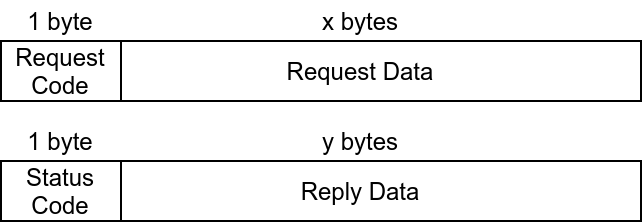
\includegraphics[width=0.6\textwidth]{figures/fig1}
    \caption{Request and reply format}
    \label{fig:fig1}
\end{figure}
